\notechapter{N-20240914}{Divisors on Curves: Zeros, Poles, and the Shape of Meromorphic Functions}

\section{Why count zeros and poles}

On a Riemann surface, a meromorphic function can have zeros and poles. Instead of listing them informally, we package them into a divisor.

A divisor is a finite formal sum
\[
  D=\sum_p n_p[p],
\]
where \(n_p\in\mathbb Z\) and only finitely many \(n_p\) are nonzero. Positive coefficients record zeros; negative coefficients record poles.

\section{Principal divisors}

For a nonzero meromorphic function \(f\), define its principal divisor by
\[
  (f)=\sum_p \operatorname{ord}_p(f)[p].
\]
This records all zeros and poles of \(f\), with multiplicity.

On the Riemann sphere, the rational function
\[
  f(z)=\frac{(z-a)^2}{z-b}
\]
has divisor
\[
  (f)=2[a]-[b]-[\infty],
\]
because the total degree of a principal divisor on a compact Riemann surface is zero.

\section{Degree}

The degree of a divisor is
\[
  \deg D=\sum_p n_p.
\]
For a principal divisor on a compact Riemann surface,
\[
  \deg(f)=0.
\]
This says that zeros and poles balance.

\section{Divisors as permissions}

A divisor \(D\) can be read as a rule for allowed poles and required zeros. Define
\[
  L(D)=\{f\text{ meromorphic}: (f)+D\ge0\}\cup\{0\}.
\]
If \(D\) is positive, it allows poles bounded by \(D\).

On \(\mathbb{CP}^1\), the space \(L(n[\infty])\) consists of polynomials of degree at most \(n\):
\[
  L(n[\infty])=\{a_0+a_1z+\cdots+a_nz^n\}.
\]
So \(\ell(n[\infty])=n+1\).

\section{Line bundles without panic}

A line bundle is a family of one-dimensional vector spaces varying over a curve. Locally it looks like \(U\times\mathbb C\), but globally the local pieces may be glued with nontrivial transition functions.

Divisors produce line bundles. The line bundle \(\mathcal O(D)\) is designed so that its sections are meromorphic functions obeying the permission rule encoded by \(D\).

This is why divisors are not merely bookkeeping. They control spaces of functions and sections.

\section{The canonical divisor}

Holomorphic \(1\)-forms also have zeros. Their divisor class is called the canonical divisor \(K\). It measures the intrinsic differential geometry of the curve.

For a compact Riemann surface of genus \(g\),
\[
  \deg K=2g-2.
\]
This number already remembers the topology of the surface.

\begin{figure}[H]
\centering
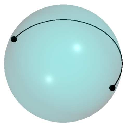
\includegraphics[width=.42\linewidth]{figures/N-20240914/1cycle.pdf}
\caption{A curve carries both topology and analytic data. Divisors are one way to connect them.}
\end{figure}

\section{Riemann--Roch as a counting theorem}

The Riemann--Roch theorem says
\[
  \ell(D)-\ell(K-D)=\deg D+1-g.
\]
This formula should not be read first as a technical spell. It is a counting theorem: it tells us how many meromorphic functions are allowed by a divisor, corrected by topology and differential forms.

For \(X=\mathbb{CP}^1\), \(g=0\), and \(D=n[\infty]\), it gives \(\ell(D)=n+1\), matching polynomials of degree at most \(n\).

\section{Hurwitz in one paragraph}

If \(f:X\to Y\) is a nonconstant holomorphic map of compact Riemann surfaces of degree \(d\), the Hurwitz formula is
\[
  2g_X-2=d(2g_Y-2)+\sum_{p\in X}(e_p-1).
\]
The integer \(e_p\) is the ramification index at \(p\). The formula says that topology changes under covering maps exactly by the ramification correction.

%% expanded-on-review

\section{Three examples on the Riemann sphere}

On \(\mathbb{CP}^1\), the function \(z-a\) has one zero at \(a\) and one pole at \(\infty\):
\[
  (z-a)=[a]-[\infty].
\]
The function \(1/(z-a)\) has divisor
\[
  \left(\frac1{z-a}\right)=-[a]+[\infty].
\]
The function \((z-a)/(z-b)\) has divisor
\[
  \left(\frac{z-a}{z-b}\right)=[a]-[b].
\]
These examples are small, but they show the whole idea: a divisor records the balance sheet of zeros and poles.

\section{Riemann--Roch on the Projective Line}

Let \(D=n[\infty]\). The condition \((f)+D\ge0\) says that \(f\) may have a pole at infinity of order at most \(n\), and no other poles. Such functions are exactly polynomials of degree at most \(n\):
\[
  1,z,z^2,\ldots,z^n.
\]
So
\[
  \ell(D)=n+1.
\]
Since \(g=0\), Riemann--Roch predicts
\[
  \ell(D)-\ell(K-D)=n+1.
\]
For \(n\ge0\), the correction term \(\ell(K-D)\) vanishes, and the formula becomes the elementary dimension count above.

This is the right way to first meet Riemann--Roch: on the sphere it says something one can already verify by hand.

\section{What not to overread}

Divisors are not a replacement for geometry. They are a language for one kind of geometric question: which functions or sections can exist with prescribed zeros and poles?

The danger is to memorize the notation while forgetting the picture. Whenever \(D\) appears, ask what behavior it permits. Whenever \(L(D)\) appears, ask which functions survive those permissions.


\section{What to remember}

Divisors turn zeros and poles into algebra. Line bundles turn divisor conditions into spaces of sections. Riemann--Roch tells us how large those spaces are.

\[
  \text{geometry asks which functions exist, and divisors say what behavior is allowed.}
\]
